\documentclass[11pt, letterpaper]{article} % Cumple Criterio 3: Equivalente al tamaño de fuente exigido

% ==========================================
% PAQUETES DE IDIOMA Y FUENTE (ARIAL 11)
% ==========================================
\usepackage[spanish, es-tabla]{babel} % es-tabla para que diga "Tabla" y no "Cuadro"
\usepackage[utf8]{inputenc}
\usepackage{helvet} % Cumple Criterio 3: Fuente similar a Arial
\renewcommand{\familydefault}{\sfdefault} % Configura la fuente sin serifas por defecto

% ==========================================
% GEOMETRÍA, INTERLINEADO Y COLUMNAS
% ==========================================
\usepackage[margin=2cm]{geometry} % Cumple Criterio 3: Márgenes exactos de 2 cm
\usepackage{setspace}
\onehalfspacing % Cumple Criterio 3: Interlineado 1.5
\usepackage{multicol} % Cumple Criterio 8: Permite doble columna a partir de la introducción

% ==========================================
% CITAS Y REFERENCIAS (NORMA APA 7)
% ==========================================
\usepackage{csquotes}
\usepackage[style=apa, backend=biber]{biblatex} % Cumple Criterio 9: Norma APA 7ma ed.
\addbibresource{referencias.bib}

% ==========================================
% TABLAS, FIGURAS Y ECUACIONES
% ==========================================
\usepackage{booktabs}
\usepackage{threeparttable}
\usepackage{graphicx}
\usepackage{tikz}
\usepackage{amsmath}
\usepackage{float}
\usepackage{caption}
\usepackage[hidelinks]{hyperref}
% Cumple Criterio 16: Figuras caption inferior, tablas caption superior
\captionsetup[table]{position=top, labelsep=period, font=normalsize}
\captionsetup[figure]{position=bottom, labelsep=period, font=normalsize}

% ==========================================
% PORTADA Y METADATOS UTS
% ==========================================
\title{
\vspace{-1.5cm} % Ajuste para subir el título y dejar espacio al logo

\includegraphics[width=8.0cm]{LOGO-UTS.png}\\[1cm]
\textbf{Separador Magnético de Residuos Metálicos con Electroimán Controlado}
}

% Cumple Criterio 2: Apellidos en mayúscula, nombres en minúscula y superíndices
\author{
  \textsc{ARIAS CAMARGO}, Juan Humberto$^{1}$; \textsc{AGUILLÓN SUÁREZ}, Johnier David$^{2}$; \\
  \textsc{GUALDRON CASTILLO}, Deisy Tatiana$^{3}$; \textsc{GÜIZA GARCIA}, Luis Alejandro$^{4}$; \\
  \textsc{PEÑA ORTIZ}, María Paula$^{5}$; \textsc{RUEDA BEDOYA}, Sebastián$^{6}$; \\
  \textsc{ROJAS CABALLERO}, Jhon Alexis$^{7}$; \textsc{RICO HERNÁNDEZ}, Saúl Alexis$^{8}$ \\[0.5cm]
  \small Unidades Tecnológicas de Santander, Departamento de Ciencias Básicas\\
  \small Electromagnetismo – E251. Docente: Iveth Vanessa Ayala Viloria\\
  \small $^{1-8}$Estudiantes de Tecnología
}
\date{4 de Octubre de 2026}

\begin{document}

\maketitle
\newpage
% ==========================================
% RESUMEN Y ABSTRACT (A UNA SOLA COLUMNA)
% ==========================================
\noindent \textbf{RESUMEN} \\
La separación manual de residuos ferromagnéticos en pequeños centros de reciclaje es lenta e ineficiente. Este proyecto tiene como objetivo diseñar y construir un separador magnético de bajo costo mediante un electroimán controlado con voltaje variable (1.5 V, 3.0 V y 4.5 V). Se utilizará alambre de cobre esmaltado (0.5 mm), núcleo de hierro, portapilas, interruptor, multímetro y dinamómetro. La metodología incluye la construcción de un electroimán de 100 vueltas, su montaje en un sistema de puente grúa manual de dos ejes (X y Z), y la medición experimental de la fuerza de atracción y la corriente. Se busca comprobar la relación teórica entre el voltaje aplicado y la capacidad de atracción del dispositivo, evaluando su viabilidad para pequeñas empresas de reciclaje. \\
\textbf{\textit{Palabras Clave:}} electromagnetismo, electroimán, separación magnética, reciclaje. % Cumple Criterio 6: Exactamente 4 palabras clave

\vspace{0.5cm}

\noindent \textbf{ABSTRACT} \\
The manual separation of ferromagnetic waste in small recycling centers is slow and inefficient. This project aims to design and build a low-cost magnetic separator using a controlled electromagnet with variable voltage (1.5 V, 3.0 V, and 4.5 V). Enameled copper wire (0.5 mm), iron core, battery holder, switch, multimeter, and dynamometer will be used. The methodology includes building a 100-turn electromagnet, mounting it on a two-axis manual bridge crane (X and Z), and the experimental measurement of the attraction force and current. The aim is to verify the theoretical relationship between the applied voltage and the attraction capacity of the device, evaluating its viability for small recycling companies. \\
\vspace{0.25cm}
\textbf{\textit{Keywords:}} electromagnetism, electromagnet, magnetic separation, recycling. % Cumple Criterio 7: Abstract y Keywords traducidos fielmente

\vspace{0.5cm}

% ==========================================
% INICIO DE DOBLE COLUMNA PARA EL CONTENIDO
% ==========================================
% Cumple Criterio 8: A partir de la Introducción a doble columna
\begin{multicols}{2}

% ==========================================
% PRIMERA ENTREGA (CORTE 1)
% PROYECTO: Separador magnético de residuos metálicos con electroimán controlado
% ==========================================

% ==========================================
% INTRODUCCIÓN
% ==========================================
\section{Introducción}

La gestión y separación eficiente de residuos sólidos constituye un pilar fundamental para optimizar los procesos de reciclaje y el aprovechamiento de materiales en la industria. En los centros de acopio a pequeña escala y en el ámbito doméstico, la clasificación de metales ferrosos suele realizarse manualmente, lo que resulta un proceso lento e ineficiente cuando estos materiales se encuentran dispersos en flujos heterogéneos compuestos por polímeros, papel y vidrio \parencite{serway2018}. Ante esta problemática, el electromagnetismo proporciona una solución tecnológica viable y de bajo costo mediante el aprovechamiento de campos magnéticos inducidos. Un electroimán, conformado por una bobina de cobre devanada alrededor de un núcleo ferromagnético, genera un campo magnético controlable al ser sometido a una corriente eléctrica; al interrumpir dicha alimentación, el núcleo pierde su magnetismo, permitiendo la liberación selectiva del material capturado \parencite{halliday2014}.

Teóricamente, la magnitud del campo magnético $B$ al interior de un solenoide con núcleo ferromagnético se modela de forma ideal mediante la Ley de Ampère generalizada:

\begin{equation}
  B = \mu_0 \mu_r \frac{N I}{L}
\end{equation}

Donde $\mu_0 = 4\pi \times 10^{-7} \, \text{T}\cdot\text{m/A}$ representa la permeabilidad magnética del vacío, $\mu_r$ la permeabilidad relativa del núcleo, $N$ el número total de espiras, $I$ la corriente eléctrica en amperios, y $L$ la longitud geométrica de la bobina. La corriente está regida por la Ley de Ohm ($I = V/R$), vinculando directamente el voltaje de alimentación $V$ con la resistencia eléctrica $R$. De acuerdo con \textcite{tipler2008}, la fuerza de atracción $F$ ejercida sobre una superficie de área transversal $A$ se expresa clásicamente como:

\begin{equation}
  F = \frac{B^2 A}{2\mu_0}
\end{equation}

No obstante, el modelo analítico anterior asume un circuito magnético ideal y cerrado. En aplicaciones reales, donde el electroimán opera en un circuito abierto (como un actuador cilíndrico atrayendo chatarra irregular), la considerable reluctancia del aire mitiga severamente el flujo magnético. Para lograr una precisión analítica superior, este proyecto incorpora la Ley de Hopkinson para circuitos magnéticos ($\mathcal{F} = \Phi \cdot \mathcal{R}_{total}$). Esta ley permite corregir el campo magnético efectivo ($B_{real}$), integrando la longitud del entrehierro y la dispersión del flujo ($l_{gap}$) en la reluctancia total del sistema \parencite{hayt2012}:

\begin{equation}
  B_{real} = \frac{\mu_0 N I}{\frac{L}{\mu_r} + l_{gap}}
\end{equation}

Al sustituir $B_{real}$ en la ecuación de fuerza, se obtiene un modelo teórico realista, respaldado en la literatura electromagnética, que atenúa las anomalías predictivas del solenoide ideal \parencite{hayt2012}.

\textbf{Pregunta de investigación.} Con base en estos principios técnicos, surge la siguiente interrogante: ¿cómo varía la fuerza de atracción de un electroimán de bajo costo en función del voltaje de alimentación (de 1 a 4 pilas en serie) y cómo incide este parámetro en la eficiencia de separación de residuos ferromagnéticos?

\textbf{Objetivo general.} Diseñar y construir un sistema de separación magnética de bajo costo que, mediante un electroimán controlado montado en un puente grúa manual, extraiga residuos metálicos ferromagnéticos de una mezcla de materiales reciclables.

% ==========================================
% OBJETIVOS ESPECÍFICOS
% ==========================================
\section{Objetivos Específicos}

\begin{itemize}
    \item \textbf{Diseñar} el componente electromagnético mediante el devanado de alambre de cobre esmaltado sobre un núcleo de acero, garantizando la generación de la fuerza de tracción magnética requerida.
    \item \textbf{Configurar} un circuito de control manual empleando fuentes de bajo voltaje para facilitar la adquisición de datos y garantizar la operación segura del sistema.
    \item \textbf{Proyectar} el diseño preliminar de un mecanismo de desplazamiento en los ejes X y Z, simulando la cinemática de un puente grúa industrial para su implementación final.
\end{itemize}

% ==========================================
% MATERIALES Y METODOLOGÍA
% ==========================================
\section{Materiales y Metodología}

% VERIFICAR el calibre del alambre en el carrete antes de entregar.
Para la fabricación del sistema electromagnético y de la futura estructura mecánica de soporte se emplearán componentes que incluyen alambre de cobre esmaltado calibre 15 AWG, un tornillo estructural de acero como núcleo ferromagnético, perfiles de madera de balso y guías tubulares de PVC para la estructura del puente grúa, un portapilas múltiple, un interruptor de balancín y conductores flexibles. La instrumentación requerida comprende un multímetro digital TM-101 Techman para la medición de voltaje y corriente, una balanza digital de precisión (resolución de 0.01 g) para la cuantificación indirecta de la fuerza de atracción, una cinta métrica convencional y un cronómetro digital.

El desarrollo metodológico se centró en la construcción, prueba y caracterización del componente electromagnético. Se ejecutó el devanado manual del alambre de cobre alrededor del núcleo hasta completar 150 espiras, asegurando el contacto eléctrico al interconectarlo en serie con el interruptor y la fuente. Los parámetros físicos consolidados del prototipo se detallan en la Tabla \ref{tab:parametros}.

\begin{table}[H]
  \centering
  \caption{\textit{Parámetros constructivos, geométricos y de modelado del electroimán.}}
  \label{tab:parametros}
  \resizebox{\linewidth}{!}{%
  \begin{tabular}{llcc}
    \hline
    \textbf{Magnitud} & \textbf{Símbolo} & \textbf{Valor} & \textbf{Origen} \\
    \hline
    Número de vueltas & $N$ & 150 & Medido \\
    Resistencia en frío & $R$ & $0.6 \, \Omega$ & Medido \\
    Longitud del devanado & $L$ & $13.2 \, \text{cm}$ & Medido \\
    Longitud del núcleo (tornillo) & $L_{Fe}$ & $14.2 \, \text{cm}$ & Medido \\
    Diámetro del núcleo & $d$ & $6.5 \, \text{mm}$ & Medido \\
    Área transversal & $A$ & $33.2 \, \text{mm}^2$ & Calculado \\
    Permeabilidad relativa & $\mu_r$ & 50 & Asumido (acero) \\
    Entrehierro efectivo inicial & $l_{gap}$ & $2.5 \, \text{mm}$ & Estimado \\
    Entrehierro efectivo calibrado & $l_{gap}$ & $1.46 \, \text{mm}$ & Ajustado (1 pila) \\
    Aceleración de la gravedad & $g$ & $9.81 \, \text{m/s}^2$ & Constante \\
    \hline
  \end{tabular}%
  }
\end{table}

Posteriormente, se procedió a la recolección de datos experimentales limitando el calentamiento del circuito. Las lecturas de corriente se tomaron restringiendo el tiempo de energización a 1 segundo y dejando un periodo de enfriamiento entre mediciones para evitar distorsiones causadas por el Efecto Joule. Se varió el voltaje en cuatro niveles (conectando de 1 a 4 pilas en serie), registrando la corriente inicial y la masa máxima de desprendimiento. De forma paralela, se estructuró el diseño planimétrico del mecanismo de desplazamiento transversal (ver Figura \ref{fig:esquema_grua}), cuya integración física se proyecta para la segunda etapa del proyecto.

\begin{figure}[H]
  \centering
  \resizebox{\linewidth}{!}{%
  \begin{tikzpicture}
    % Bandeja 1: Residuos Mezclados
    \draw[thick, fill=gray!10, rounded corners] (0,0) rectangle (4.9,1);
    \node[align=center, font=\small\bfseries, text width=8cm] at (2.45,0.5) {Bandeja de Residuos\\[-4pt]Mezclados};

    % Bandeja 2: Residuos Separados
    \draw[thick, fill=gray!20, rounded corners] (5.1,0) rectangle (10,1);
    \node[align=center, font=\small\bfseries, text width=8cm] at (7.55,0.5) {Bandeja de Residuos\\[-4pt]Separados};

    % Columnas de soporte (Madera)
    \draw[thick, fill=brown!50] (0.5, 1) rectangle (1.2, 7);
    \draw[thick, fill=brown!50] (8.8, 1) rectangle (9.5, 7);

    % Riel longitudinal (Tubo PVC)
    \draw[thick, fill=gray!30] (1.2, 6) rectangle (8.8, 6.4);
    \node[above] at (1.8, 6.4) {Riel de PVC (Eje X)};

    % Travesaño móvil (Madera o PVC) con ruedas/deslizador
    \draw[thick, fill=brown!70] (4.2, 5.8) rectangle (5.8, 6.8);
    \draw[<->, ultra thick, blue] (2.5, 7.2) -- (7.5, 7.2) node[midway, above] {Movimiento Horizontal (X)};

    % Mecanismo vertical (Eje Z)
    \draw[thick, fill=gray!60] (4.8, 3.5) rectangle (5.2, 6);
    \draw[<->, ultra thick, blue] (3.8, 3.5) -- (3.8, 5.5) node[midway, left] {Eje Z};

    % Electroimán (Núcleo y Bobina)
    \draw[thick, fill=gray!80] (4.7, 2) rectangle (5.3, 3.5); % Núcleo de hierro
    \draw[thick, fill=orange!60, rounded corners=1pt] (4.4, 2.2) rectangle (5.6, 3.3); % Bobina de cobre

    % Simulación de espiras de alambre
    \foreach \y in {2.3, 2.5, 2.7, 2.9, 3.1}
      \draw (4.4, \y) -- (5.6, \y);

    \node[right] at (5.7, 2.75) {Bobina (150 vueltas)};
    \node[right] at (5.4, 1.8) {Núcleo de acero};

    % Líneas de campo magnético esquemáticas
    \draw[->, dashed, red] (4.5, 1.9) .. controls (4, 1) and (6, 1) .. (5.5, 1.9);
  \end{tikzpicture}%
  }
  \caption{\textit{Diseño preliminar de elevación frontal del puente grúa manual. Se ilustra la cinemática de desplazamiento proyectada para la fase experimental.}}
  \label{fig:esquema_grua}
\end{figure}

Para el procesamiento de los datos se elaboró una memoria de cálculos en la que se determinaron, para cada configuración de voltaje, la resistencia efectiva, la potencia disipada, la fuerza de atracción y el campo magnético (tanto experimentales como teóricos), incluyendo sus respectivos errores absoluto y relativo. Los cálculos se estructuraron en tres escenarios: las mediciones experimentales directas, un modelo teórico base fundamentado en la Ley de Hopkinson con un entrehierro efectivo estimado en $2.5 \, \text{mm}$, y un modelo teórico mejorado.

En ambos modelos teóricos se empleó la corriente medida en cada configuración. En el modelo mejorado, la longitud del entrehierro efectivo ($l_{gap}$) se calibró con los datos de la primera configuración (1.54 V), asumiendo que en este nivel se presenta la menor influencia de saturación magnética; dicho valor se aplicó constante al resto de las configuraciones. El procesamiento y la ilustración gráfica de los datos se desarrollaron en lenguaje Python, empleando las bibliotecas NumPy y Pandas para el análisis numérico, y Seaborn para la visualización.

% ==========================================
% RESULTADOS Y DISCUSIÓN
% ==========================================
\section{Resultados y Discusión}

El análisis del comportamiento electromagnético del prototipo se fundamentó en las características físicas del devanado y del núcleo (Tabla \ref{tab:parametros}). A partir de estos parámetros, el comportamiento dinámico se evaluó contrastando los datos experimentales (Tabla \ref{tab:datos_exp}) con las dos aproximaciones teóricas formuladas. Los valores y los márgenes de error se resumen en la Tabla \ref{tab:datos_teo} y se representan en las Figuras \ref{fig:graficas_log} y \ref{fig:grafica_error}.

\begin{table}[H]
  \centering
  \caption{\textit{Datos experimentales de voltaje, corriente y fuerza de atracción.}}
  \label{tab:datos_exp}
  \resizebox{\linewidth}{!}{%
  \begin{tabular}{cccccc}
    \hline
    \textbf{Pilas} & \textbf{Voltaje} & \textbf{Corriente} & \textbf{Masa} & \textbf{Fuerza (Exp)} & \textbf{Campo (Exp)}\\
     & \textbf{(V)} & \textbf{(A)} & \textbf{(g)} & \textbf{(N)} & \textbf{(T)}\\
    \hline
    1 & 1.54 & 1.82 & 8.58 & 0.0842 & 0.0798 \\
    2 & 3.08 & 2.09 & 13.41 & 0.1316 & 0.0998 \\
    3 & 4.62 & 2.93 & 14.23 & 0.1396 & 0.1028 \\
    4 & 6.16 & 3.19 & 15.70 & 0.1540 & 0.1080 \\
    \hline
  \end{tabular}%
  }
  \vspace{2pt}
  \footnotesize{\textit{Nota.} La fuerza se calculó como $F = m g$ y el campo experimental como $B = \sqrt{2\mu_0 F/A}$.}
\end{table}

\begin{table}[H]
  \centering
  \caption{\textit{Valores teóricos y errores frente a la medición experimental.}}
  \label{tab:datos_teo}
  \resizebox{\linewidth}{!}{%
  \begin{tabular}{lcccc}
    \hline
    \textbf{Magnitud} & \textbf{1.54 V} & \textbf{3.08 V} & \textbf{4.62 V} & \textbf{6.16 V} \\
    \hline
    \multicolumn{5}{l}{\textit{Caracterización eléctrica}} \\
    $R$ efectiva ($\Omega$) & 0.85 & 1.47 & 1.58 & 1.93 \\
    Potencia (W) & 2.80 & 6.44 & 13.54 & 19.65 \\
    \hline
    \multicolumn{5}{l}{\textit{Modelo base ($l_{gap} = 2.5 \, \text{mm}$)}} \\
    $F$ teórica (N) & 0.0545 & 0.0719 & 0.1412 & 0.1674 \\
    Error absoluto $F$ (N) & -0.0297 & -0.0597 & 0.0016 & 0.0134 \\
    Error relativo $F$ (\%) & -35.26 & -45.38 & 1.17 & 8.69 \\
    $B$ teórico (T) & 0.0642 & 0.0738 & 0.1034 & 0.1126 \\
    Error absoluto $B$ (T) & -0.0156 & -0.0260 & 0.0006 & 0.0046 \\
    Error relativo $B$ (\%) & -19.54 & -26.09 & 0.58 & 4.26 \\
    \hline
    \multicolumn{5}{l}{\textit{Modelo mejorado ($l_{gap} = 1.46 \, \text{mm}$)}} \\
    $F$ teórica (N) & 0.0842 & 0.1110 & 0.2181 & 0.2586 \\
    Error relativo $F$ (\%) & 0.00 & -15.63 & 56.27 & 67.89 \\
    $B$ teórico (T) & 0.0798 & 0.0917 & 0.1285 & 0.1399 \\
    Error relativo $B$ (\%) & 0.00 & -8.14 & 25.01 & 29.57 \\
    \hline
  \end{tabular}%
  }
  \vspace{2pt}
  \footnotesize{\textit{Nota.} Error relativo $= (\text{teórico} - \text{experimental})/\text{experimental} \times 100$. La resistencia en frío medida de la bobina fue de $0.6 \, \Omega$; el incremento de la resistencia efectiva ($R = V/I$) es consistente con la disipación térmica por Efecto Joule. Los modelos usan la corriente medida. El 0.00\,\% a 1.54 V es resultado de la calibración del entrehierro con esa configuración.}
\end{table}

\begin{figure}[H]
  \centering
  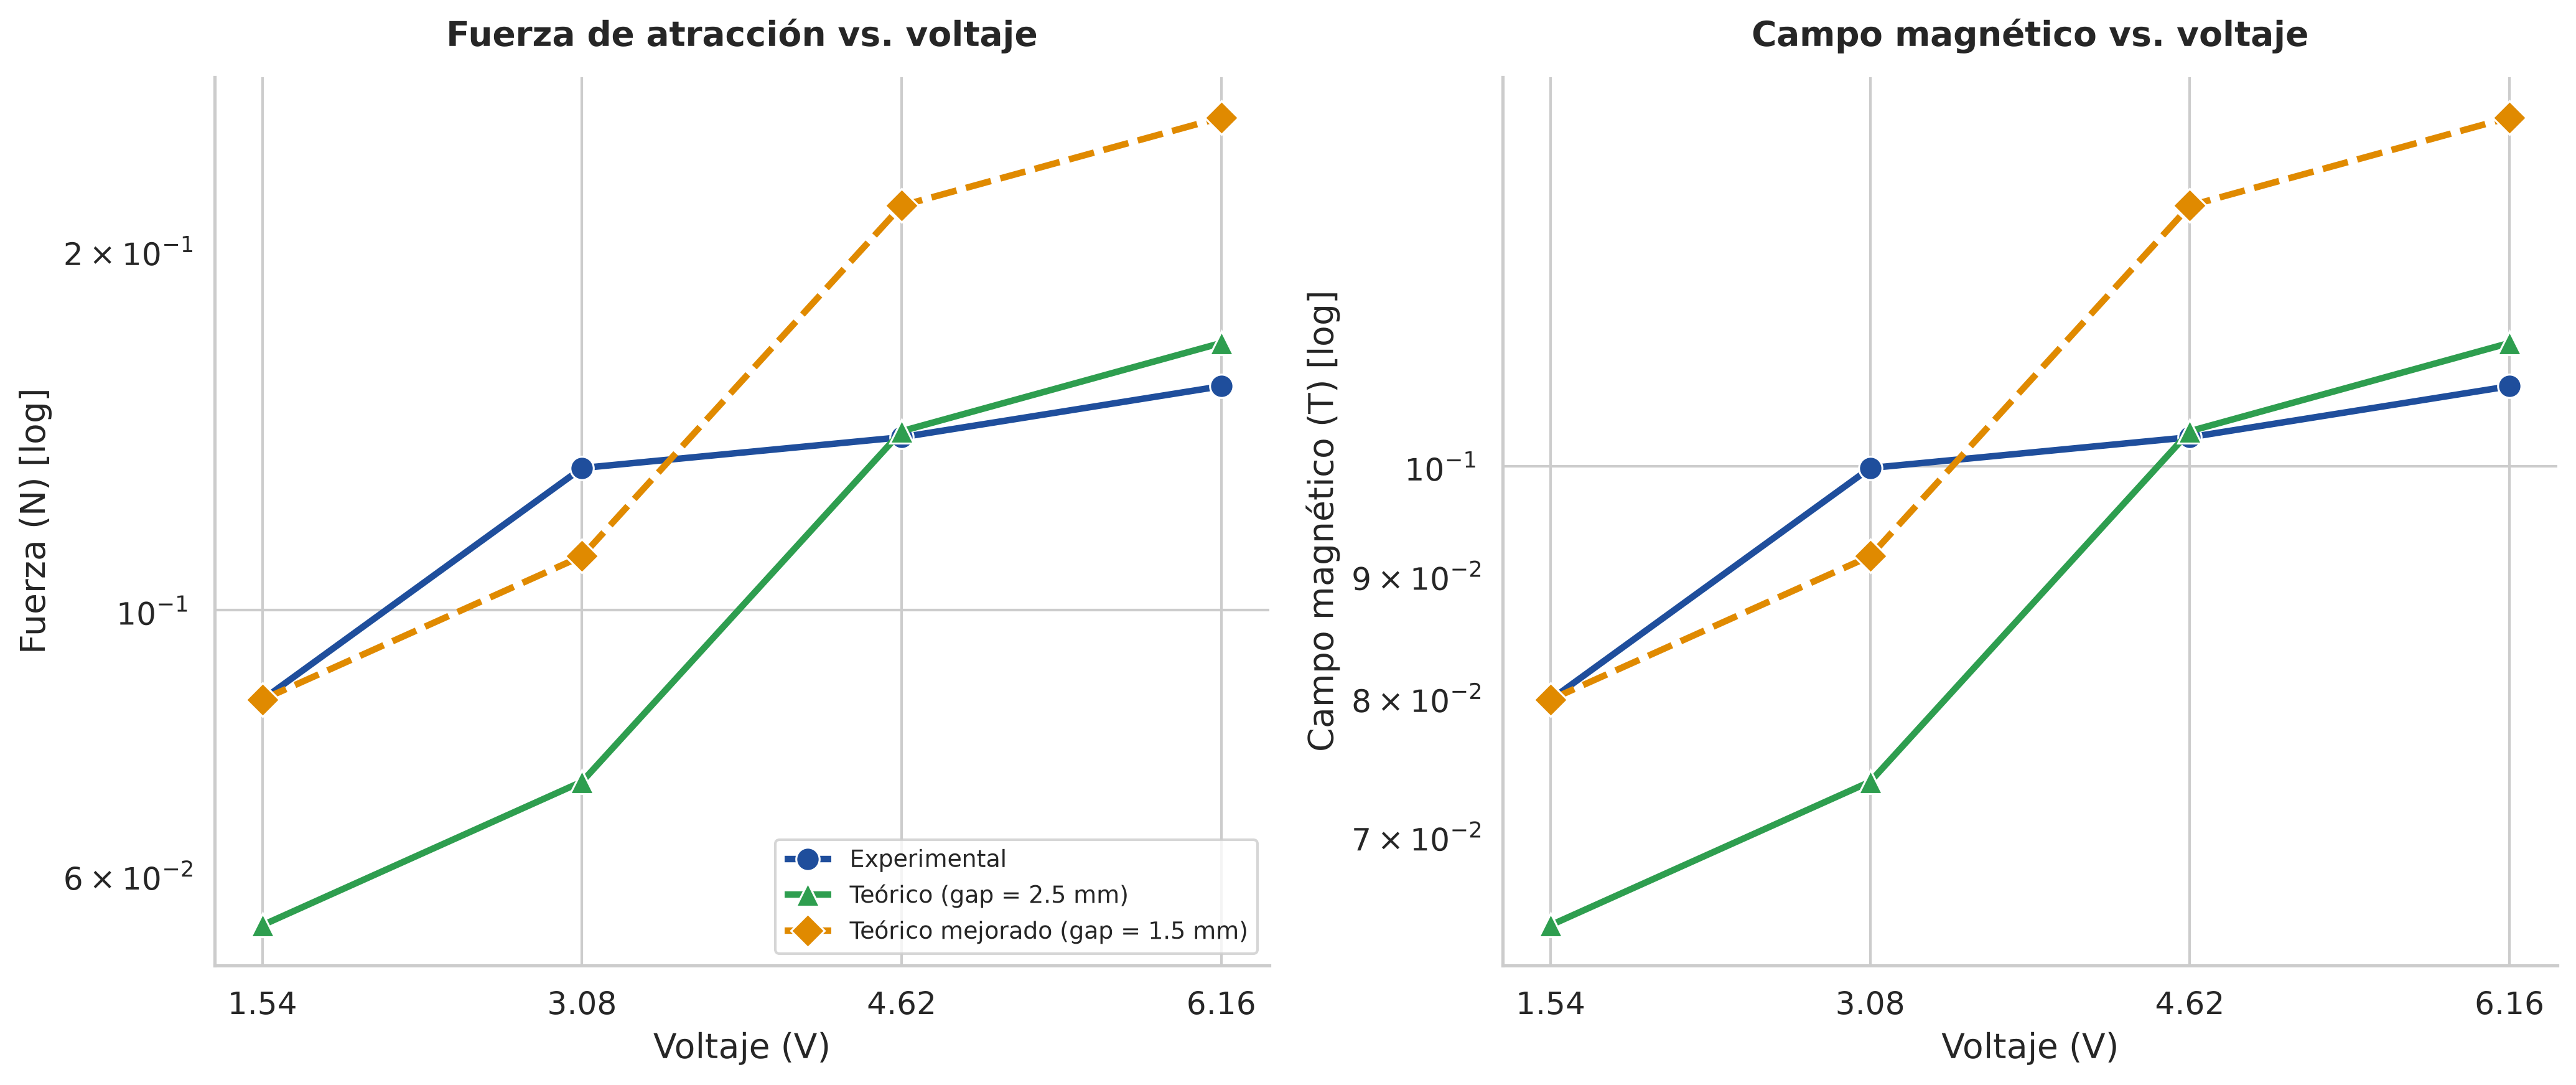
\includegraphics[width=0.95\linewidth]{grafica_1_log.png}
  \caption{\textit{Comparación de Fuerza de Atracción y Campo Magnético en escala logarítmica frente a la variación de voltaje.}}
  \label{fig:graficas_log}
\end{figure}

\begin{figure}[H]
  \centering
  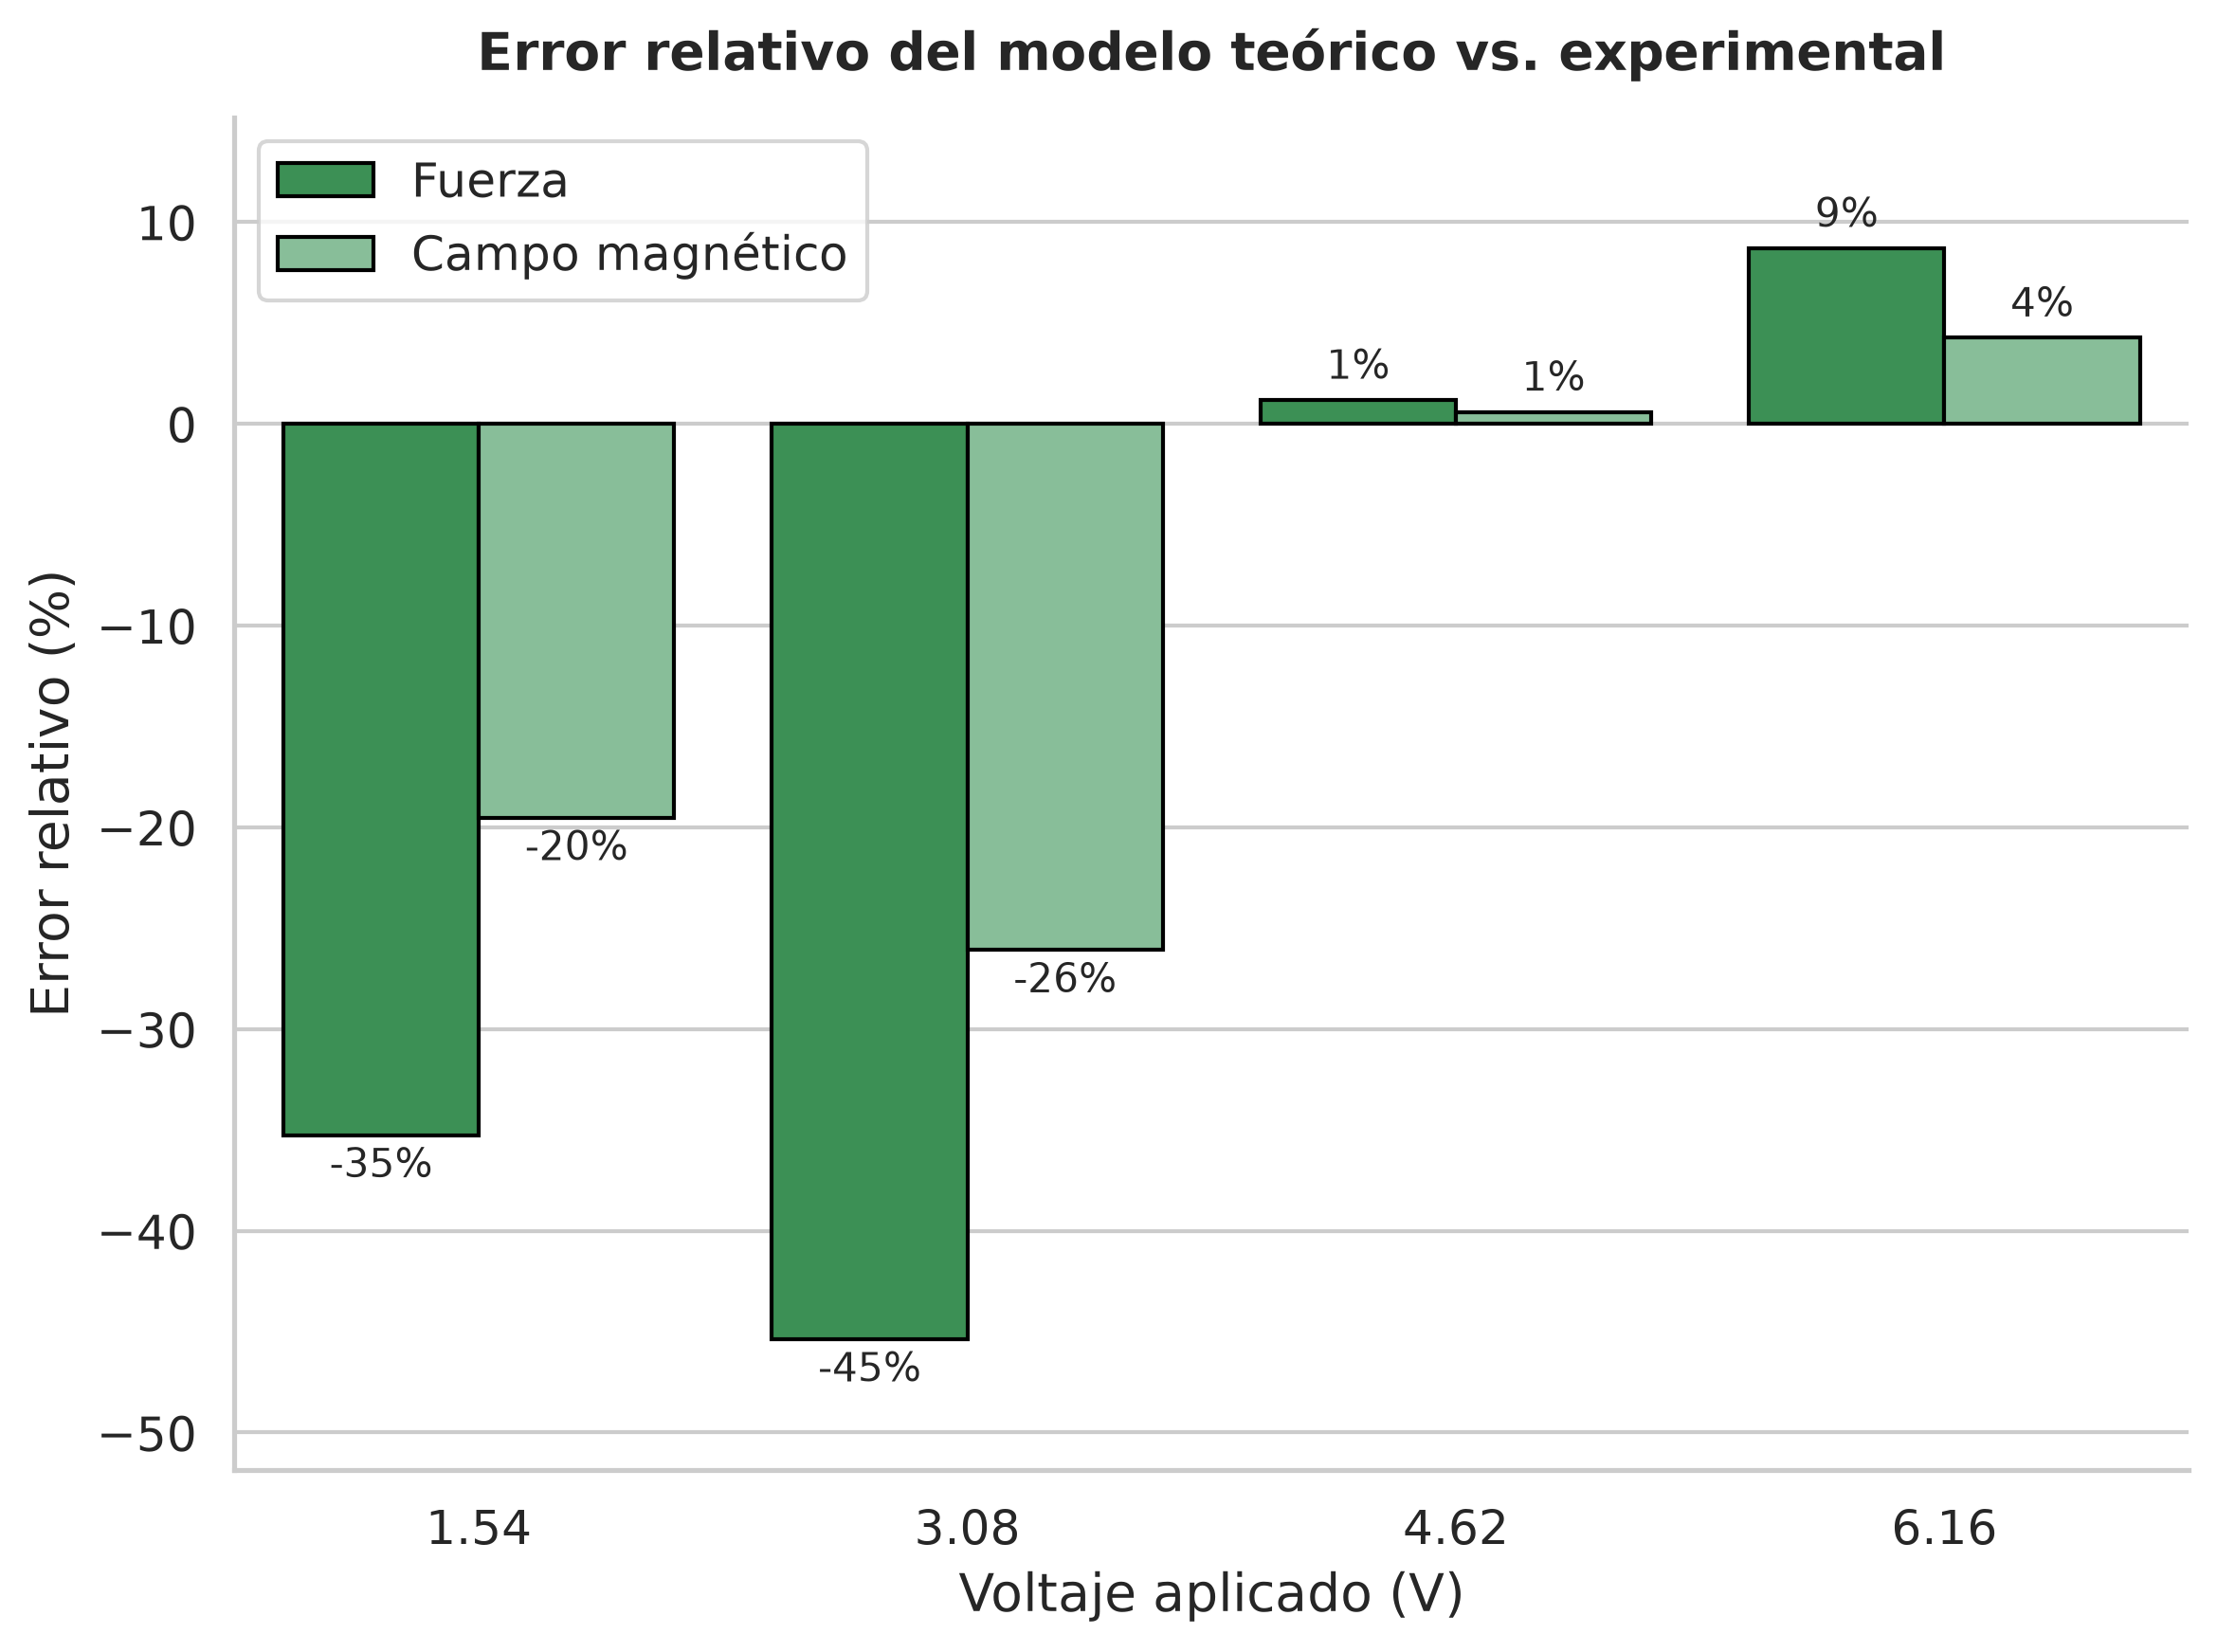
\includegraphics[width=0.9\linewidth]{grafica_2_error.png}
  \caption{\textit{Evolución del error relativo porcentual frente al incremento de tensión aplicada.}}
  \label{fig:grafica_error}
\end{figure}

Como se observa en la Tabla \ref{tab:datos_teo}, la resistencia efectiva del circuito ($R = V/I$) aumentó de $0.85 \, \Omega$ en la configuración inicial (1 pila) a $1.93 \, \Omega$ con 4 pilas. Este incremento, acompañado de un crecimiento acelerado de la potencia disipada (hasta 19.65 W), es consistente con el Efecto Joule, junto con la resistencia interna de las pilas y de los contactos, que no se midieron por separado. En conjunto, estos factores impidieron que la corriente mantuviera un comportamiento lineal respecto al voltaje, y actuaron como un factor limitante de la escalabilidad de la fuerza de tracción.

Adicionalmente, el modelo base (con un entrehierro estimado de $2.5 \, \text{mm}$, no ajustado a los datos) subestima la fuerza de atracción con 1 y 2 pilas (errores de $-35.3$\% y $-45.4$\%) y se aproxima con 3 y 4 pilas ($+1.2$\% y $+8.7$\%); en el campo magnético los errores son de $-19.5$\%, $-26.1$\%, $+0.6$\% y $+4.3$\% (ver Figura \ref{fig:grafica_error}). La discrepancia es más pronunciada en la fuerza que en el campo, dado que $F$ es proporcional al cuadrado de $B$. El modelo mejorado, con el entrehierro calibrado en la primera configuración ($1.46 \, \text{mm}$), reproduce la fuerza con dos pilas con un error de $-15.6$\%, pero la sobrestima con 3 y 4 pilas (56.3\% y 67.9\%). El 0\% de la primera configuración es consecuencia de la calibración y no un resultado de validación.

Ambos modelos predicen un campo proporcional a la corriente, mientras que el campo experimental crece menos que ella: la relación $B/I$ cae de 0.044 y 0.048 T/A con 1 y 2 pilas a 0.035 y 0.034 T/A con 3 y 4 pilas. Por eso el signo del error cambia con la corriente en ambos modelos, y la cercanía del modelo base con 3 y 4 pilas se debe al valor de entrehierro elegido y no a que describa mejor la física. Este comportamiento sublineal sugiere saturación magnética del núcleo, junto con el aumento de la dispersión del flujo y el calentamiento: entre 4.62 V y 6.16 V, la fuerza experimental solo aumentó de 0.1396 N a 0.1540 N, a pesar de que la potencia disipada pasó de 13.54 W a 19.65 W.

La superposición de la disipación térmica y la saturación magnética impide aislar sus contribuciones individuales con los datos registrados, y tampoco permite afirmar que alguno de los dos modelos sea superior en todo el rango; su cuantificación queda planteada para la fase experimental siguiente. Los fenómenos cualitativos observados durante la experimentación se consolidan en la Tabla \ref{tab:observaciones}.

\begin{table}[H]
  \centering
  \caption{\textit{Observaciones cualitativas experimentales.}}
  \label{tab:observaciones}
  \begin{tabular}{@{}p{0.25\linewidth} p{0.68\linewidth}@{}}
    \hline
    \textbf{Ensayo} & \textbf{Observación Física} \\
    \hline
    1 Pila \newline(1.54 V) & Desprendimiento fácil de los residuos. La corriente medida presentó alta estabilidad inicial.\\
    2 Pilas \newline(3.08 V) & Mejora notable en la adherencia. Se detectó un leve calentamiento en el alambre tras unos segundos.\\
    3 Pilas \newline(4.62 V) & Atracción fuerte. La corriente comenzó a decaer rápidamente debido a la disipación por Efecto Joule.\\
    4 Pilas \newline(6.16 V) & Posible saturación. La resistencia interna limitó el pico a 3.19 A frente a los 10.27 A teóricos. Se requirió enfriamiento.\\
    \hline
  \end{tabular}
\end{table}

% ==========================================
% APLICACIÓN EN EL ENTORNO
% ==========================================
\section{Aplicación en el Entorno de la Comunidad}

Aunque la estructura mecánica del separador se encuentra en fase de proyección conceptual, los principios electromagnéticos caracterizados en esta primera etapa evidencian un alto potencial de transferencia tecnológica al contexto local. El dispositivo emula a escala los principios operativos de los separadores magnéticos industriales.

Para una cooperativa local de recicladores o centros de acopio municipales, la integración de este componente sobre un sistema de traslación automatizado (como un puente grúa o una banda transportadora) permitiría aislar metales ferrosos con mayor rapidez. Esta tecnificación impactaría positivamente en la salud ocupacional, al mitigar riesgos mecánicos y biológicos asociados a la manipulación manual de chatarra, y optimizaría los tiempos de procesamiento en flujos de residuos altamente heterogéneos.

% ==========================================
% CONCLUSIONES
% ==========================================
\section{Conclusiones}

La fuerza de atracción del prototipo mostró una dependencia no lineal respecto al voltaje de alimentación. Al cuadruplicar el voltaje (de 1.54 V a 6.16 V), la fuerza solo aumentó un factor de 1.8 (de 0.0842 N a 0.1540 N), mientras que la potencia disipada pasó de 2.80 W a 19.65 W. En consecuencia, la relación fuerza/potencia decreció de aproximadamente 0.030 N/W a 0.008 N/W. Entre 2 y 4 pilas, la fuerza aumentó cerca de 17\% mientras la potencia se triplicó, lo que indica que, para la geometría y los materiales empleados, alimentar con más de dos pilas aporta ganancias marginales de fuerza a cambio de una mayor disipación y calentamiento. Estos resultados responden a la primera parte de la pregunta de investigación; su incidencia sobre la eficiencia de separación en condiciones reales se abordará en la fase de ensamble final.

En términos de modelado, la Ley de Hopkinson con un entrehierro efectivo reprodujo el orden de magnitud de la fuerza, pero ninguno de los dos modelos, lineales en la corriente, describió el comportamiento sublineal del prototipo: el modelo base ($2.5 \, \text{mm}$, estimado) subestimó la fuerza con 1 y 2 pilas ($-35$\% y $-45$\%) y se aproximó con 3 y 4, mientras que el modelo mejorado ($1.46 \, \text{mm}$, calibrado con la primera configuración) quedó en $-15.6$\% con dos pilas y sobrestimó con 3 y 4. El entrehierro efectivo es un parámetro de ajuste que agrupa la separación real, la dispersión y el retorno del flujo en un circuito abierto, y no una longitud medida; además, el error nulo de la primera configuración no constituye una validación. Las desviaciones a mayor corriente sugieren que el modelo requeriría incorporar la curva de magnetización $B$--$H$ del núcleo para describir la saturación. Como trabajo futuro, se propone repetir los ensayos de cada configuración, estimar el entrehierro con separaciones conocidas entre el núcleo y la pieza atraída, y evaluar la separación sobre flujos heterogéneos de residuos.


El video técnico en el que los integrantes explican el proyecto se encuentra disponible en el siguiente enlace: \url{https://drive.google.com/drive/folders/1wp3MN6vj4wUwwEoGPDJDvJUMf2JtGP_P?usp=sharing}.

% ==========================================
% AGRADECIMIENTOS
% ==========================================
\section*{Agradecimientos}

Los autores agradecen a la docente del curso de Electromagnetismo de las Unidades Tecnológicas de Santander por su orientación durante el desarrollo del proyecto, y a quienes brindaron apoyo y espacios para la construcción y las pruebas del prototipo.

% ==========================================
% ANEXOS
% ==========================================
\section{Anexos}

Se presenta el registro fotográfico del prototipo y del trabajo experimental (Figuras \ref{fig:anexo1}, \ref{fig:anexo2} y \ref{fig:anexo3}).

\begin{figure}[H]
  \centering
  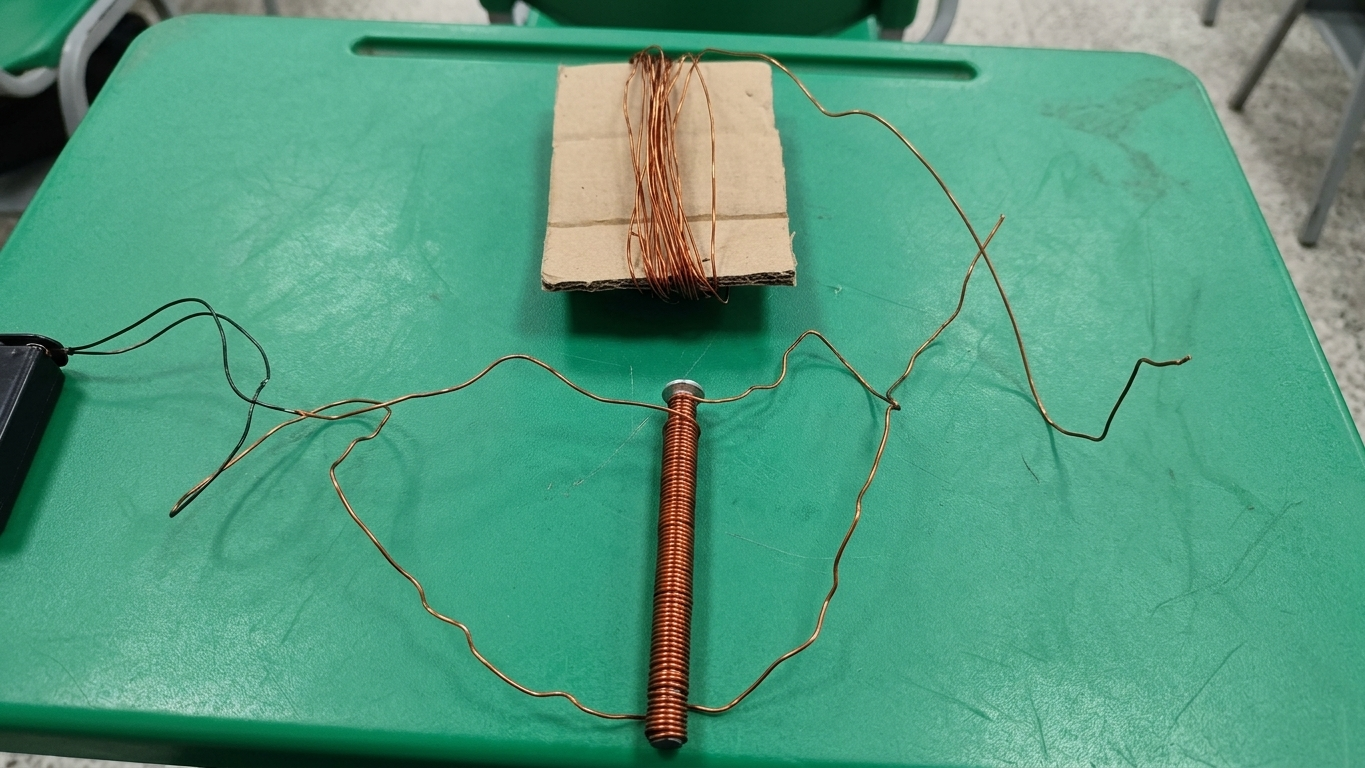
\includegraphics[width=0.85\linewidth]{Anexos/A1_Electroiman-ya-embobinado.jpeg}
  \caption{\textit{Electroimán ya embobinado. Fuente: elaboración propia.}}
  \label{fig:anexo1}
\end{figure}

\begin{figure}[H]
  \centering
  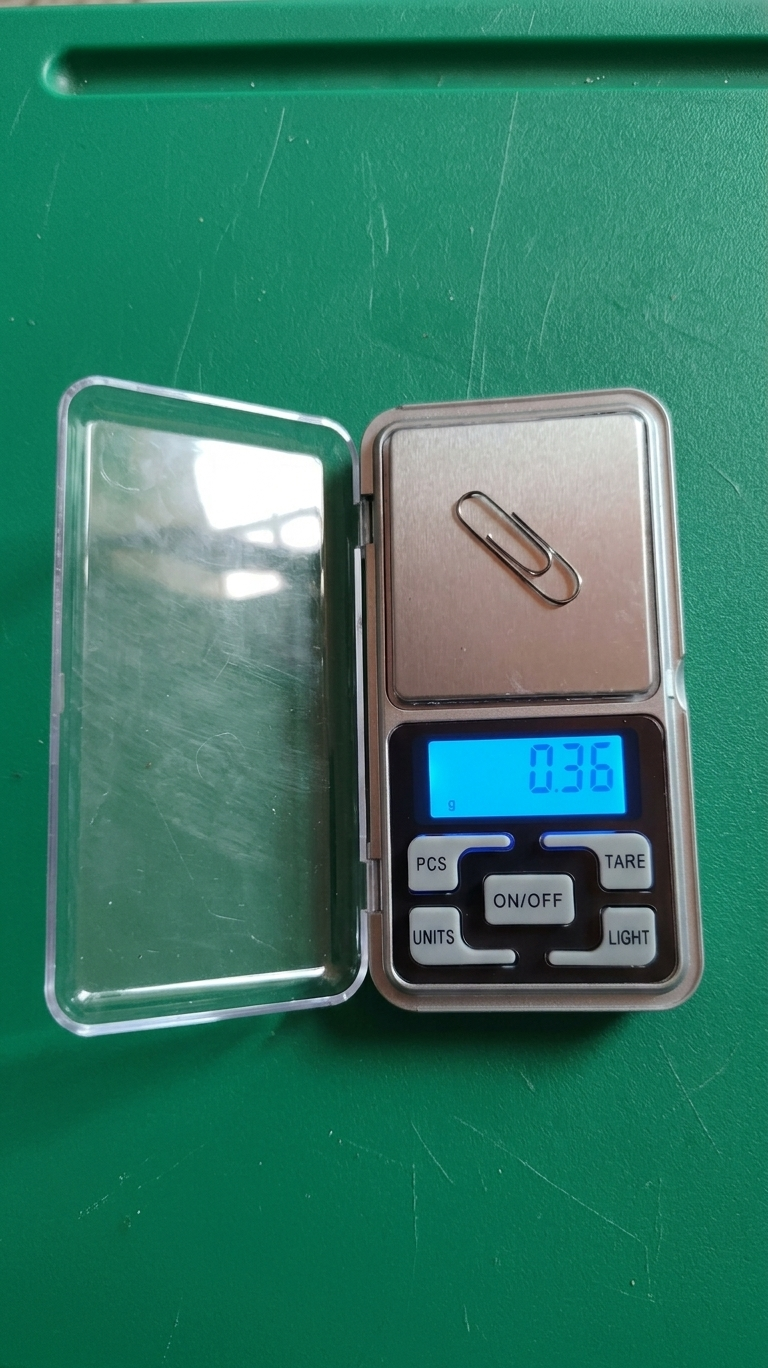
\includegraphics[width=0.85\linewidth]{Anexos/A2_gramera-pesando-clip.jpeg}
  \caption{\textit{Balanza digital pesando un clip, carga utilizada en la prueba (cada clip pesa 1.36 g). Fuente: elaboración propia.}}
  \label{fig:anexo2}
\end{figure}

\begin{figure}[H]
  \centering
  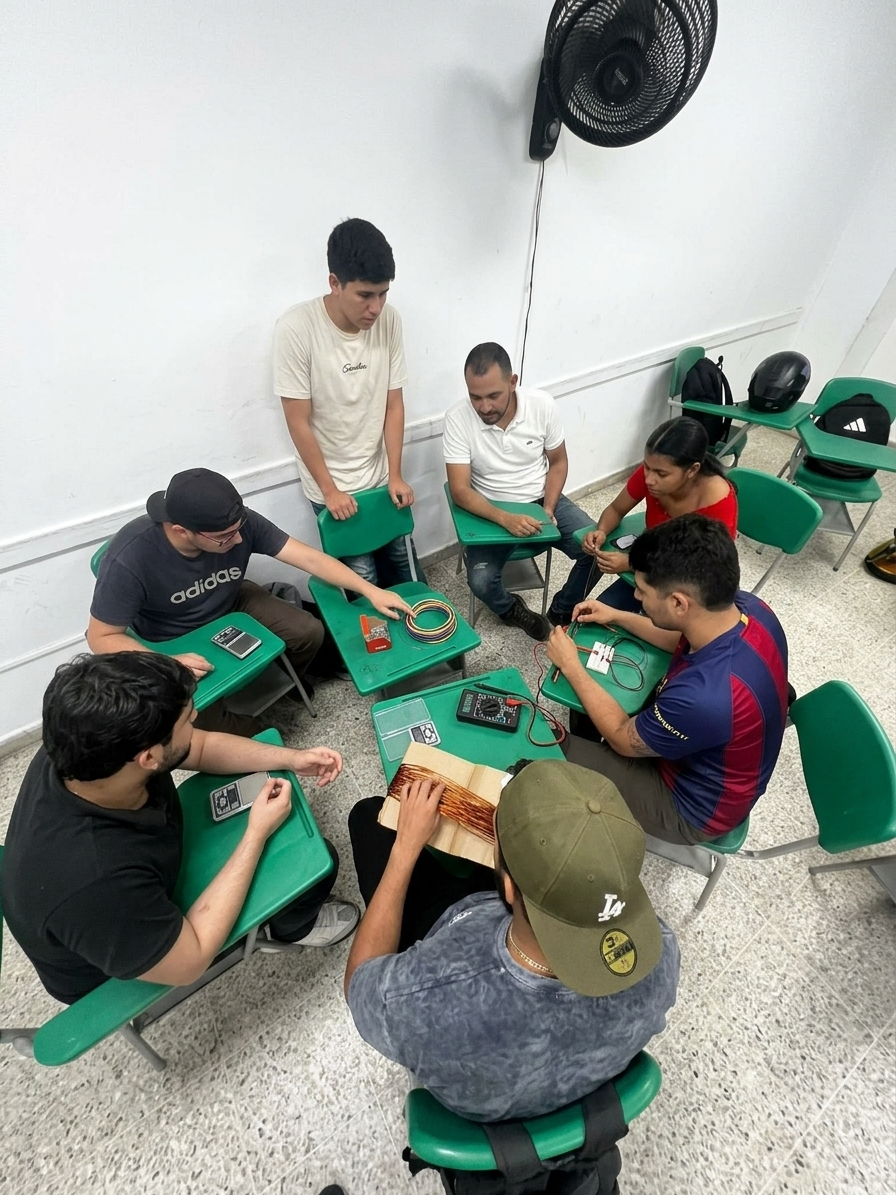
\includegraphics[width=0.85\linewidth]{Anexos/A3_Equipo-de-trabajo-con-materiales.jpeg}
  \caption{\textit{Equipo de trabajo con los materiales del proyecto. Fuente: elaboración propia.}}
  \label{fig:anexo3}
\end{figure}


\nocite{*} % Incluye todas las referencias del .bib aunque no se citen en el texto
\printbibliography

\end{multicols}

\end{document}
